\documentclass[a4paper,12pt,french]{article}

\usepackage[cours]{../../../Style}

%\usepackage[theorems]{tcolorbox}

%\newtcbtheorem
%{defi}{Définition}
%{colback=red!5,colframe=red!60!black!80,fonttitle=
%\sffamily\bfseries}{th}

% Début du document
%%%%%%%%%%%%%%%%%%%
\begin{document}

\title{Fonctions polynômiales de degré 2}
\maketitle

\begin{programme}
\item représentations graphiques des fonctions : $x \mapsto ax^2,x \mapsto ax^2+b, x \mapsto a(x-x_1)(x-x_2)$
\item axes de symétrie ;
\item racines et signe d'un polynôme de degré 2 donné sous forme factorisée (le calcul des
racines à l'aide du discriminant ne figure pas au programme).
\item Compétences
\begin{itemize}
\item Associer une parabole à une expression algébrique de degré 2
\item Déterminer des éléments caractéristiques de la fonction $x \mapsto a(x-x_1)(x-x_2)$: Signe, extremum, allure, axes de symétrie
\item Vérifier qu'une valeur conjecturée est racine d'un polynôme de degré 2
\item Savoir factoriser dans des cas simples une expression du second degré connaissant une racine.
\item Utiliser la forme factorisée d'un poly pour trouver ses racines et étudier son signe.
\end{itemize}
\item déterminer le signe d'une expression factorisée du second degré
\item résoudre une équation ou une inéquation du premier degré, une équation du type $x^2=a$ avec $a \geq 0$.
\end{programme}

\section{Généralités}

\begin{defin}
On appelle fonction polynômiale de degré $2$ toute fonction $$\fonction f {\R} {\R} x {ax^2+bx+c}$$ Où $a,\ b,\ c \in \R$ et $a \neq 0$.
\end{defin}

\begin{exs}
$f:x \mapsto x^2 \ , \ g:x \mapsto 3x^2-4$ et $h:x \mapsto 2-0,3x^2$ sont des fonctions polynômiales de degré 2.
\end{exs}

\rem{Fonctions polynômiales de degré 2 un peu lourd... On dira plutôt polynômes de degré 2 même si ce n'est techniquement pas tout à fait le même objet}

\rem{Prévoir exo: reconnaitre $a,b,c$}

\section{Fonctions $x \mapsto ax^2+b$}

\rem[eleve]{On s'intéresse maintenant à des cas plus simples. Les propositions suivantes sont généralisables.}

\begin{prop}
La représentation graphique d'une fonction polynômiale du second degré est une parabole.
\end{prop}

\begin{exs}
\begin{centrer}
\begin{tikzpicture}[scale=\echellepgf]
\begin{axis}[
styleglobal,
hauteurproptick,
width=0.7*\echellepgfinv*\linewidth,
xmin=-7, xmax=7,
ymin=-4.5, ymax=6,
xtick distance=1,
ytick distance=1,
domain=(-6:6),
]
\addplot[styleplot]{x^2} node[pos=0.55,right] {$\mathscr C_f$};
\addplot[color=red,styleplot]{3*x^2-4} node[pos=0.545,left] {$\mathscr C_g$};
\addplot[color=blue,styleplot]{2-0.25*x^2} node[pos=0.8,right] {$\mathscr C_h$};
\end{axis}
\end{tikzpicture}
\end{centrer}
\end{exs}

\rem{Montrer sur geogebra l'effet obtenu en changeant $a$ et $b$}

\begin{rmq}
$b$ est l'ordonnée à l'origine de la parabole. Changer $b$ décale la parabole vers le haut ou vers le bas.
\end{rmq}

\begin{proprs}
Soit $f:x \mapsto ax^2+b$ avec $a \neq 0$.
\begin{itemize}
\item Si $a \geq 0$,  $f$ est décroissante puis croissante: elle branche vers le haut.
\item Si $a \leq 0$,  $f$ est croissante puis décroissante: elle branche vers le bas.
\end{itemize}
\end{proprs}

\begin{defin}
On appelle sommet d'une parabole le point où elle change de direction. C'est le point le plus bas si $a > 0$, le point le plus haut sinon.

\begin{centrer}
\begin{tikzpicture}[scale=\echellepgf]
\begin{axis}[
styleglobal,
hauteurproptick,
width=0.7*\echellepgfinv*\linewidth,
xmin=-4, xmax=4,
ymin=-1.5, ymax=1.5,
xtick distance=1,
ytick distance=1,
domain=(-6:6),
]
\addplot[styleplot]{1-x^2} node[pos=0.53,right] {$\mathscr C_f$};
\node[stylepoint,fill=red] (S) at (0,1) {};
\node (sommet) at (1,1.2) {Sommet};
\draw[->,>=latex] (sommet.west) to[bend right=10] (S);
\end{axis}
\end{tikzpicture}
\end{centrer}

\end{defin}

\begin{proprs}
Soit $f:x \mapsto ax^2+b$ avec $a \neq 0$.
\begin{itemize}
\item Les paraboles d'équation $y=ax^2+b$ ont pour axe de symétrie l'axe des ordonnées.
\item Le sommet de la parabole associée est le point $(0;b)$.
\end{itemize}
\end{proprs}

\rem{Exos 20,21,23 p120}

\begin{methode}
Pour déterminer l'expression d'une fonction $f:x \mapsto ax^2+b$ à partir de sa représentation graphique, on lit d'abord $b$ en regardant l'ordonnée à l'origine, puis on détermine $a$ en résolvant une équation.
\end{methode}

\begin{ex}
\compo[0.7]
{
On a représenté $f:x \mapsto ax^2+b$ sur le repère ci-contre.

\

On voit directement que $b=1$, d'où $f:x \mapsto ax+1$.

\

On se donne maintenant un point sur la courbe de $f$, par exemple $A(1;3)$. Cela signifie que $f(1)=3$, autrement dit $a \times 1 + 1=3$, soit donc $a+1=3$, d'où $a=2$.

\

On a alors $f:x \mapsto 2x^2+1$.
}
{
\vspace{-9mm}
\begin{centrer}
\begin{tikzpicture}[scale=\echellepgf]
\begin{axis}[
styleglobal,
hauteurproptick,
width=0.9*\echellepgfinv*\linewidth,
xmin=-2.5, xmax=2.5,
ymin=-0.5, ymax=5,
xtick distance=1,
ytick distance=1,
domain=(-6:6),
]
\addplot[styleplot]{2*x^2+1} node[pos=0.52,right] {$\mathscr C_f$};
\node at (0,1) {};
\end{axis}
\end{tikzpicture}
\end{centrer}
}
\end{ex}

\rem{Exo 22p121, prévoir un autre exo du type sur fiche}

\section{Fonctions $x \mapsto a(x-x_1)(x-x_2)$}
\subsection{Généralités}

\begin{prop}
Les fonctions du type $f:x \mapsto a(x-x_1)(x-x_2)$ sont des fonctions polynômiales du second degré.
\end{prop}

\begin{fait}
En effet, $\begin{aligned}[t]a(x-x_1)(x-x_2) & =a(x^2-xx_2-xx_1+x_1x_2) \\ & =ax^2-axx_2-axx_1+ax_1x_2 \\ & =ax^2-(ax_1+ax_2)x+ax_1x_2 \end{aligned}$

Donc $a(x-x_1)(x-x_2) =a x^2+b x + c$ avec $b = -(ax_1+ax_2)$ et $c=ax_1x_2$.
\end{fait}

\begin{defin}
Soit $f$ une fonction polynômiale de degré 2. On appelle \textbf{racines} de $f$ les solutions de l'équation $f(x)=0$. Ce sont donc les abscisses des points d'intersection entre la courbe représentative de $f$ et l'axe des abscisses.
\end{defin}

\begin{rmq}
Si $f(x)=a(x-x_1)(x-x_2)$ $(a \neq 0)$, les racines de $f$ sont $x_1$ et $x_2$.
\end{rmq}

\begin{fait}
En effet, $\begin{aligned}[t] a(x-x_1)(x-x_2)=0 & \Leftrightarrow a=0 \text{ ou } x-x_1=0 \text{ ou } x-x_2=0 \\ & \Leftrightarrow x=x_1 \text{ ou } x=x_2 \end{aligned}$
\end{fait}

\begin{ex}
Les racines de la fonction $f:x \mapsto -3(x-2)(x+4)$ sont 2 et $-4$.
\end{ex}

\rem{Exos 84,85 p125}

\begin{proprs}
Soit $f:x \mapsto a(x-x_1)(x-x_2)$ avec $a \neq 0$.
\begin{itemize}
\item On pose $s=\frac{x_1+x_2} 2$. Le sommet de la parabole associée a pour coordonnées $(s,f(s))$.
\item La parabole associée a pour axe de symétrie la droite parallèle a l'axe des ordonnées (verticale) passant par son sommet.
\item On en déduit le tableau de variations de $f$:

\compo
{
\begin{center}
Si $a>0$:
\begin{tikzpicture}
\tkzTabInit[lgt=1.2,espcl=2.5]{$x$ /1, $f(x)$/2}{$- \infty$, $s$, $+ \infty$}
\tkzTabVar{+/$+ \infty$, -/ $f(s)$, +/ $+\infty$}
\end{tikzpicture}
\end{center}
}
{
\begin{center}
Si $a<0$:
\begin{tikzpicture}
\tkzTabInit[lgt=1.2,espcl=2.5]{$x$ /1, $f(x)$/2}{$- \infty$, $s$, $+ \infty$}
\tkzTabVar{-/$- \infty$, +/ $f(s)$, -/ $-\infty$}
\end{tikzpicture}
\end{center}
}
\end{itemize}

\begin{centrer}
\begin{tikzpicture}[scale=\echellepgf]
\begin{axis}[
styleglobal,
hauteurproptick,
width=0.7*\echellepgfinv*\linewidth,
xmin=-2, xmax=6,
ymin=-1, ymax=2,
xtick distance=1,
ytick distance=1,
domain=(-6:6),
]
\addplot[styleplot]{0.5*(x-1)*(x-3)} node[pos=0.52,right] {$\mathscr C_f$};
\node[stylepoint,fill=red] (S) at (2,-0.5) {};
\node (sommet) at (3,-0.7) {Sommet};
\draw[->,>=latex] (sommet.west) to[bend left=10] (S);
\node[stylepoint,fill=blue] (x1) at (1,0) {};
\node[stylepoint,fill=blue] (x2) at (3,0) {};
\node (racines) at (2,1) {Racines};
\draw[->,>=latex] (racines) to[bend right=10] (x1);
\draw[->,>=latex] (racines) to[bend left=10] (x2);
\end{axis}
\end{tikzpicture}
\end{centrer}

\end{proprs}

\rem{Exos 26,27,29 p121}

\subsection{Factorisation}

\begin{fait}
Soit $f:x \mapsto ax^2+b+c$. On souhaite retrouver l'écriture factorisée $f(x)=a(x-x_1)(x-x_2)$.
\end{fait}

\begin{methode}
Si l'on connait une racine $x_1$ de $f$, on peut retrouver l'écriture factorisée de $f$ par identification.
\end{methode}

\begin{ex}
Soit $f:x \mapsto x^2-3x+2$. Cherchons d'abord une racine dite "évidente" de $f$.

On remarque que $f(1)=0$ donc on peut prendre $x_1=1$.

On sait alors qu'on peut écrire $f(x)=a(x-1)(x-x_2)$ avec $a,x_2 \in \R$.

Développons cette expression: $\begin{aligned}[t]f(x)&=a\left( x^2-x \times x_2-x+x_2 \right)\\&= {\color{DarkRed}a}x^2+{\color{DarkGreen}(a-ax_2)}x+{\color{DarkBlue}ax_2}\end{aligned}$

On a de plus $f(x)={\color{DarkRed}1} x^2 {\color{DarkGreen}-3}x+{\color{DarkBlue}2}$.

On a alors $\left\{ \begin{aligned} &{\color{DarkRed}a=1} \\ &{\color{DarkGreen}a-ax_2=-3} \\ &{\color{DarkBlue}ax_2=2} \end{aligned} \right.$ donc $a=1$ et $ax_2=2 \Rightarrow x_2=2$.

On en déduit que $f(x)=1(x-1)(x-2)=(x-1)(x-2)$.
\end{ex}

\begin{rmq}
Le $a$ qui apparait dans la forme développée et factorisée est le même!
\end{rmq}

\begin{ex}
Soit $f:x \mapsto 3x^2-9x+6$. On a $a=3$ donc la forme développée de $f$ sera de la forme $f(x)=3(x-x_1)(x-x_2)$.
\end{ex}

\begin{rems}
Prévoir exos de factorisation \\
Exos 60 -> 66 p123 \\
Exo 28 p121
\end{rems}

\subsection{Etude du signe}

\begin{rmq}
Une fonction du type $f:x \mapsto a(x-x_1)(x-x_2)$ peut être vue comme un produit d'un nombre réel et de deux fonctions affines.
\end{rmq}

\begin{methode}
Pour dresser algébriquement le tableau de signes d'une fonction du type $f:x \mapsto a(x-x_1)(x-x_2)$, on peut étudier le signe des deux fonctions affines qui la composent et d'utiliser la règle des signes.
\end{methode}

\begin{ex}
Soit $f:x \mapsto 0,5(x-1)(x+3)$. Cette fonction est donc composée des deux fonctions affines $x \mapsto x-1$ et $x \mapsto x+3$. On peut d'abord dresser le tableau de signes de ces deux fonctions:

\compo[0.5]
{
\begin{center}
\begin{tikzpicture}
\tkzTabInit[lgt=1.2,espcl=2]{$x$ /1, $x-1$/1}{$- \infty$, $1$, $+ \infty$}
\tkzTabLine{,-,z,+,}
\end{tikzpicture}
\end{center}
}
{
\begin{center}
\begin{tikzpicture}
\tkzTabInit[lgt=1.2,espcl=2]{$x$ /1, $x+3$/1}{$- \infty$, $-3$, $+ \infty$}
\tkzTabLine{,-,z,+,}
\end{tikzpicture}
\end{center}
}

\

On peut alors combiner ces tableaux pour dresser le tableau de signes de $f$:

\begin{centrer}
\begin{tikzpicture}
\tkzTabInit[lgt=3]{$x$ /1, $x-1$/1, $x+3$/1,$(x-1)(x+3)$/1,$f(x)$/1}{$- \infty$, $-3$, $1$, $+ \infty$}
\tkzTabLine{,-,t,-,z,+}
\tkzTabLine{,-,z,+,t,+}
\tkzTabLine{,+,z,-,z,+}
\tkzTabLine{,+,z,-,z,+}
\end{tikzpicture}
\end{centrer}


On peut vérifier que l'on obtient le même tableau par lecture graphique.

\begin{centrer}
\begin{tikzpicture}[scale=\echellepgf]
\begin{axis}[
styleglobal,
width=0.6*\echellepgfinv*\linewidth,
xmin=-8, xmax=6,
ymin=-3, ymax=5,
domain=(-6:6),
]
\addplot[styleplot]{0.5*(x-1)*(x+3)} node[pos=0.52,right] {$\mathscr C_f$};
\node at (0,1) {};
\end{axis}
\end{tikzpicture}
\end{centrer}

\end{ex}

\begin{rems}
Prévoir exos \\
Exos 72 -> 74 p124
\end{rems}
\end{document}
